\documentclass[../menv_main.tex]{subfiles}
 
\newcommand\tab[1][1.5cm]{\hspace*{#1}}

\begin{document}

\section{Introduction}

MENV can be run from the command line (``clmenv.m") or GUI (``menv.m"). The GUI and original MENV functions were written by Hui Li. Kiersten added the command line functionality, and copied over much of Hui Li's original code into \verb|clmenv|. 

\section{Envelope integrator}

MENV integrates the KV envelope equations in X and Y:

\begin{equation}
X''=-K_X X - \frac{2\mathit{K}}{X+Y} + \frac{E_X^2}{X^3}
\end{equation}

The integration is handled in the Matlab function ``menv\_integrator," which integrates through a specified beam-line given focusing gradients. The integration uses the leap-frog method. The two sub-functions which form each integration step are given below:

\begin{lstlisting}[language=Matlab]
function [x2,y2,xp2,yp2,d2,dp2] = step(x1,y1,xp1,yp1,d1,dp1)
	% function for single step
	x2 = x1+xp1*ds;
	y2 = y1+yp1*ds;
	d2 = d1+dp1*ds;
	[xpp,ypp,dpp] = calc_prim2(x2,y2,d2);
	xp2 = xp1+xpp*ds;
	yp2 = yp1+ypp*ds;
	dp2 = dp1+dpp*ds;
end
\end{lstlisting}

\begin{lstlisting}[language=Matlab]
function [xpp1,ypp1,dpp1] = calc_prim2(x1,y1,d1)
	% function to calculate velocity impulse
	% Reiser eq. 4.191, 4.192
	xpp1 = -( kx*x1-2*K/(x1+y1)-Ex^2/(x1^3) );
	ypp1 = -( ky*y1-2*K/(x1+y1)-Ey^2/(y1^3) );
	dpp1 = irho - kx*d1;
end
\end{lstlisting}

\subsubsection{Edge Focusing}

Special consideration of dipole edge-focusing has to be made to accurately model UMER dynamics. In MENV, the edge focusing term is included as a hard-edged quadrupole with the same length as the dipole. The strength is not set automatically (ie, by setting a bend-angle), but an appropriate number must be determined by the user. 
 
MENV allows for an asymmetry to be built into the horizontal and vertical edge-focusing, as separate gradient arrays are stored for each plane (\verb|KX| and \verb|KY|). The vertical focusing strength is set to the value chosen by the user for the quadrupole gradient strength at the dipole, while the horizontal focusing is defined as a scalar times this value. By default, the multiplicative factor is set to 0. No net horizontal focusing will be applied, following the argument that geometric focusing perfectly cancels the edge-defocusing in a sector dipole. 

If you want to include the additional horizontal focusing observed in UMER dipoles due to sextupole terms (Kishek, R., \& Cornacchia, M. (2010). Tech. Note, Modeling of UMER Dipoles.), you will need to change the scaling parameter \verb|Dffx| that appears around line 30 in ``menv\_makekappaarray.m".

\section{Running MENV from the GUI}

The GUI can be launched by executing the command \verb|menv| from the Matlab command line. Prior to running MENV, make sure that all files in the MENV directory are in the Matlab path (run \verb|setpath| from the command line). This will launch a GUI window as shown in Fig. \ref{fig:main}.

\begin{figure}
\centering
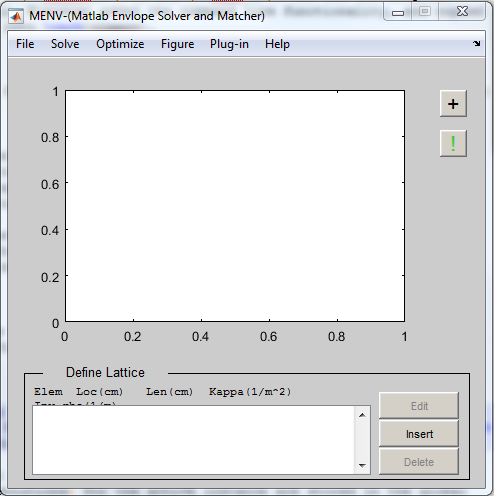
\includegraphics{figures/main_gui_window.png}
\caption{Main GUI window as it appears after launching MENV.}
\label{fig:main}
\end{figure}

\subsubsection{Defining and solving a lattice}



\begin{figure}
\centering
\includegraphics{figures/defElement_window.png}
\caption{GUI window for inserting new elements.}
\label{fig:defelement}
\end{figure}

\begin{figure}
\centering
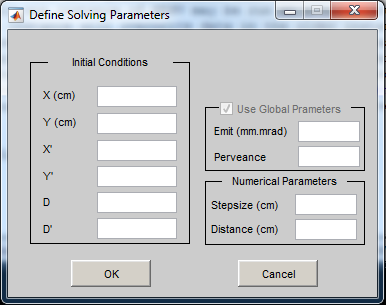
\includegraphics{figures/defparam_window.png}
\caption{GUI window for defining beam parameters.}
\label{fig:defparam}
\end{figure}


Elements can be added using the ``Insert" button, through a GUI interface shown in Fig. \ref{fig:defelement}. Beam parameters (including initial conditions, emittance and perveance) are defined using the ``Beam Parameters" option in the ``Solve" drop-down menu. This launches the GUI shown in Fig. \ref{fig:defparam}. Alternatively, run-files with .spt extension can be loaded using the command ``Open" in the drop-down menu (or Ctrl-O). 

Once beam and lattice parameters are defined, you can solve the envelope equations by hitting the solve button (green exclamation mark) or selecting ``Compute Solution" from the ``Solve" menu. To draw a schematic of the lattice elements, press the ``draw" button. 
Figure \ref{fig:fodo} shows the solution for a 0.7 mA beam in a FODO lattice defined in the example file ``FODO\_0\_7mA\_dipl.spt." 

\begin{figure}
\centering
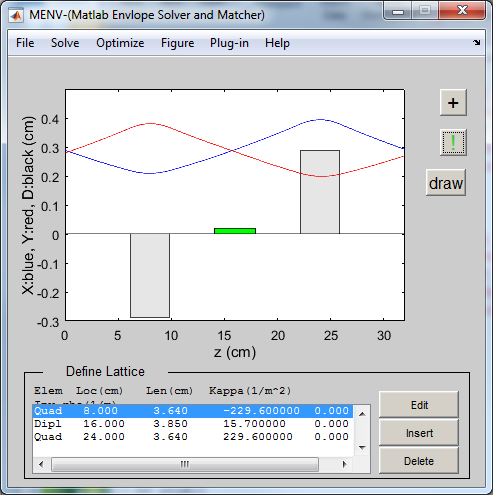
\includegraphics{figures/maingui_fodo.png}
\caption{FODO lattice solution from example file ``FODO\_0\_7mA\_dipl.spt."}
\label{fig:fodo}
\end{figure}

\clearpage
\subsubsection{Optimization in the GUI}

MENV allows for two kinds of optimization: optimizing over initial beam conditions to find the periodic solution and optimizing quadrupole/solenoid strengths to meet a target condition. Before running a matching routine, you must define targets and weights by selecting ``Matcher Parameters" under ``Optimize." The GUI that is launched is shown in Fig. \ref{fig:defmatcher}. If you are optimizing for the periodic solution, only the weights need to be defined. 
If you are optimizing to a target, targets must be defined as well. Targets and weights for X,Y,X',Y' at the end of the transport line must always be defined. 

There are additional targets and weights that \textit{may} be defined as desired; if not defined they will be set to a default value of 0. Optional targets include desired values of X and Y tunes. Optional weights include dispersion (use if you want to also find the periodic solution for dispersion), weights for the tune condition, and weights for global properties of the beam envelope. The global properties include a condition for ``roundness" \verb|X=Y|, which is defined as the rms value of \verb|x(s)-y(s)| along the beam-line. The \verb|Ref Traj| condition tries to match the envelope to a reference trajectory (inspired by the SPOT code, on which MENV is based [Allen, C. K., Guharay, S. K., \& Reiser, M. (1998). Optimal Transport of low Energy Particle Beams. Epac, (3), 2324–2326.]). The reference trajectory is defined either by loading a text file in which a curve is defined as series of points in X-Z (``Plug-in," ``Reference Trajectory," ``Load") or by drawing in the MENV window (``Plug-in," ``Reference Trajectory," ``Draw"). 

\begin{figure}
\centering
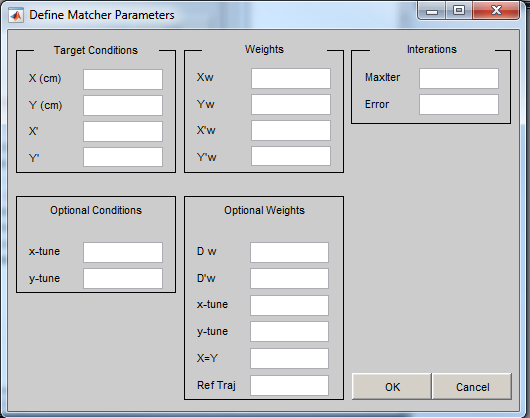
\includegraphics{figures/defmatcher_window.png}
\caption{GUI window for defining parameters for matching/optimization routines.}
\label{fig:defmatcher}
\end{figure}

\subsubsection{Side note on parallel instances}
The data (parameters, settings and solutions) for the active instance are stored in the global object \verb|guim|. As this is a global variable that does not have a unique name for each instance of MENV, only one instance of MENV may be run at a time (you can launch two, but data from the most recent instance will overwrite data in the older instance). If you want to run parallel MENV instances, you need to run separate Matlab instances as well. This could be resolved by attaching data to the GUI window rather than a global variable, and this was the case in the older (Hui Li) version of MENV. The choice was made to adopt a global variable to allow use of functions written in the ``command-line" MENV class \verb|clmenv| from within the GUI (instead of having separate functions for command-line and GUI versions).


\end{document}



